\section{Galaxy Redshift Surveys}
\label{sec:surveys}
Many of the cosmological probes (e.g. SNIa, BAO, LSS, etc., see section~\ref{sec:cosmo_model}) involve measuring the 3D position on the sky of large amounts of celestial objects such as galaxies. Therefore, observations of large areas of the sky must be carried out to provide photometry or spectroscopy of those objects and, thus, measure their cosmological redshift. These observation campaigns are known as galaxy redshift surveys and, nowadays, there are a wide range of them depending on the area they survey, the depth, etc. In this thesis we refer to several of them: the 2-degree Field Galaxy Redshift Survey (2dFGRS), the Sloan Digital Sky Survey (SDSS) and the Physics of the Accelerating Universe at the William Herschel Telescope (PAU@WHT) Survey.

\subsection{2-degree Field Galaxy Redshift Survey (2dFGRS)}
\label{sec:2df}
The 2dF Galaxy Redshift Survey (2dFGRS) \citep{Colless2001} was a spectroscopic survey conducted by the Anglo-Australian Observatory (AAO) with the 3.9~m Anglo-Australian telescope (left of Fig.~\ref{fig:2df_survey}) between 1997 and 2002. At the time, it was the second largest redshift survey, next to the Sloan Digital Sky Survey (next subsection). The 2dF survey covered an area of about 1500~sq.~deg. of the sky, surveying regions in both the north and the south galactic poles.

The 2dF instrument (right of Fig.~\ref{fig:2df_survey}) was installed at the primary focus permitting the observation of a field of 2~deg per pointing, what gives the name to the survey. The instrument possessed a spectrograph equipped with two banks each of 200 optical fibers\footnote{Optical fibers are used to provide multiobject spectroscopy simultaneously in a single exposure. Each fiber is placed on the focal plane to capture the light of the projected image of a single target. Then, this light is redirected to a dispersing element that produces the spectra.}, permitting the simultaneous measurement of 400 spectra.

The data from this survey were made public on 30 June 2003 and consist of photometry of 382323 objects, from which 245591 include spectra. Out of spectra, 232155 are galaxies (221414 with good quality spectra), 12311 are stars, and 125 are quasi-stellar objects (quasars). The survey needed 272 nights of observation, during 5 years. 
\begin{figure}
\centering
\begin{tabular}{rl}
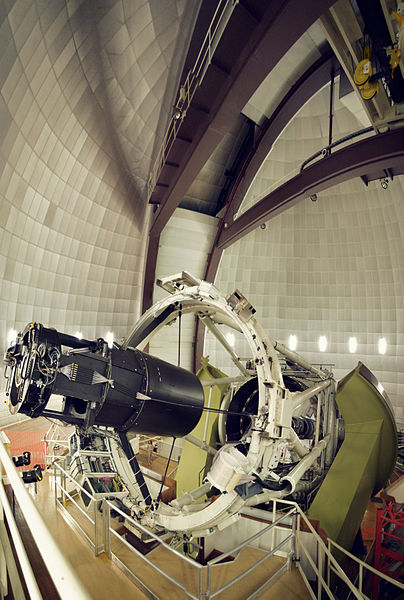
\includegraphics[height=50mm]{./plots/2df_camera.jpg} & 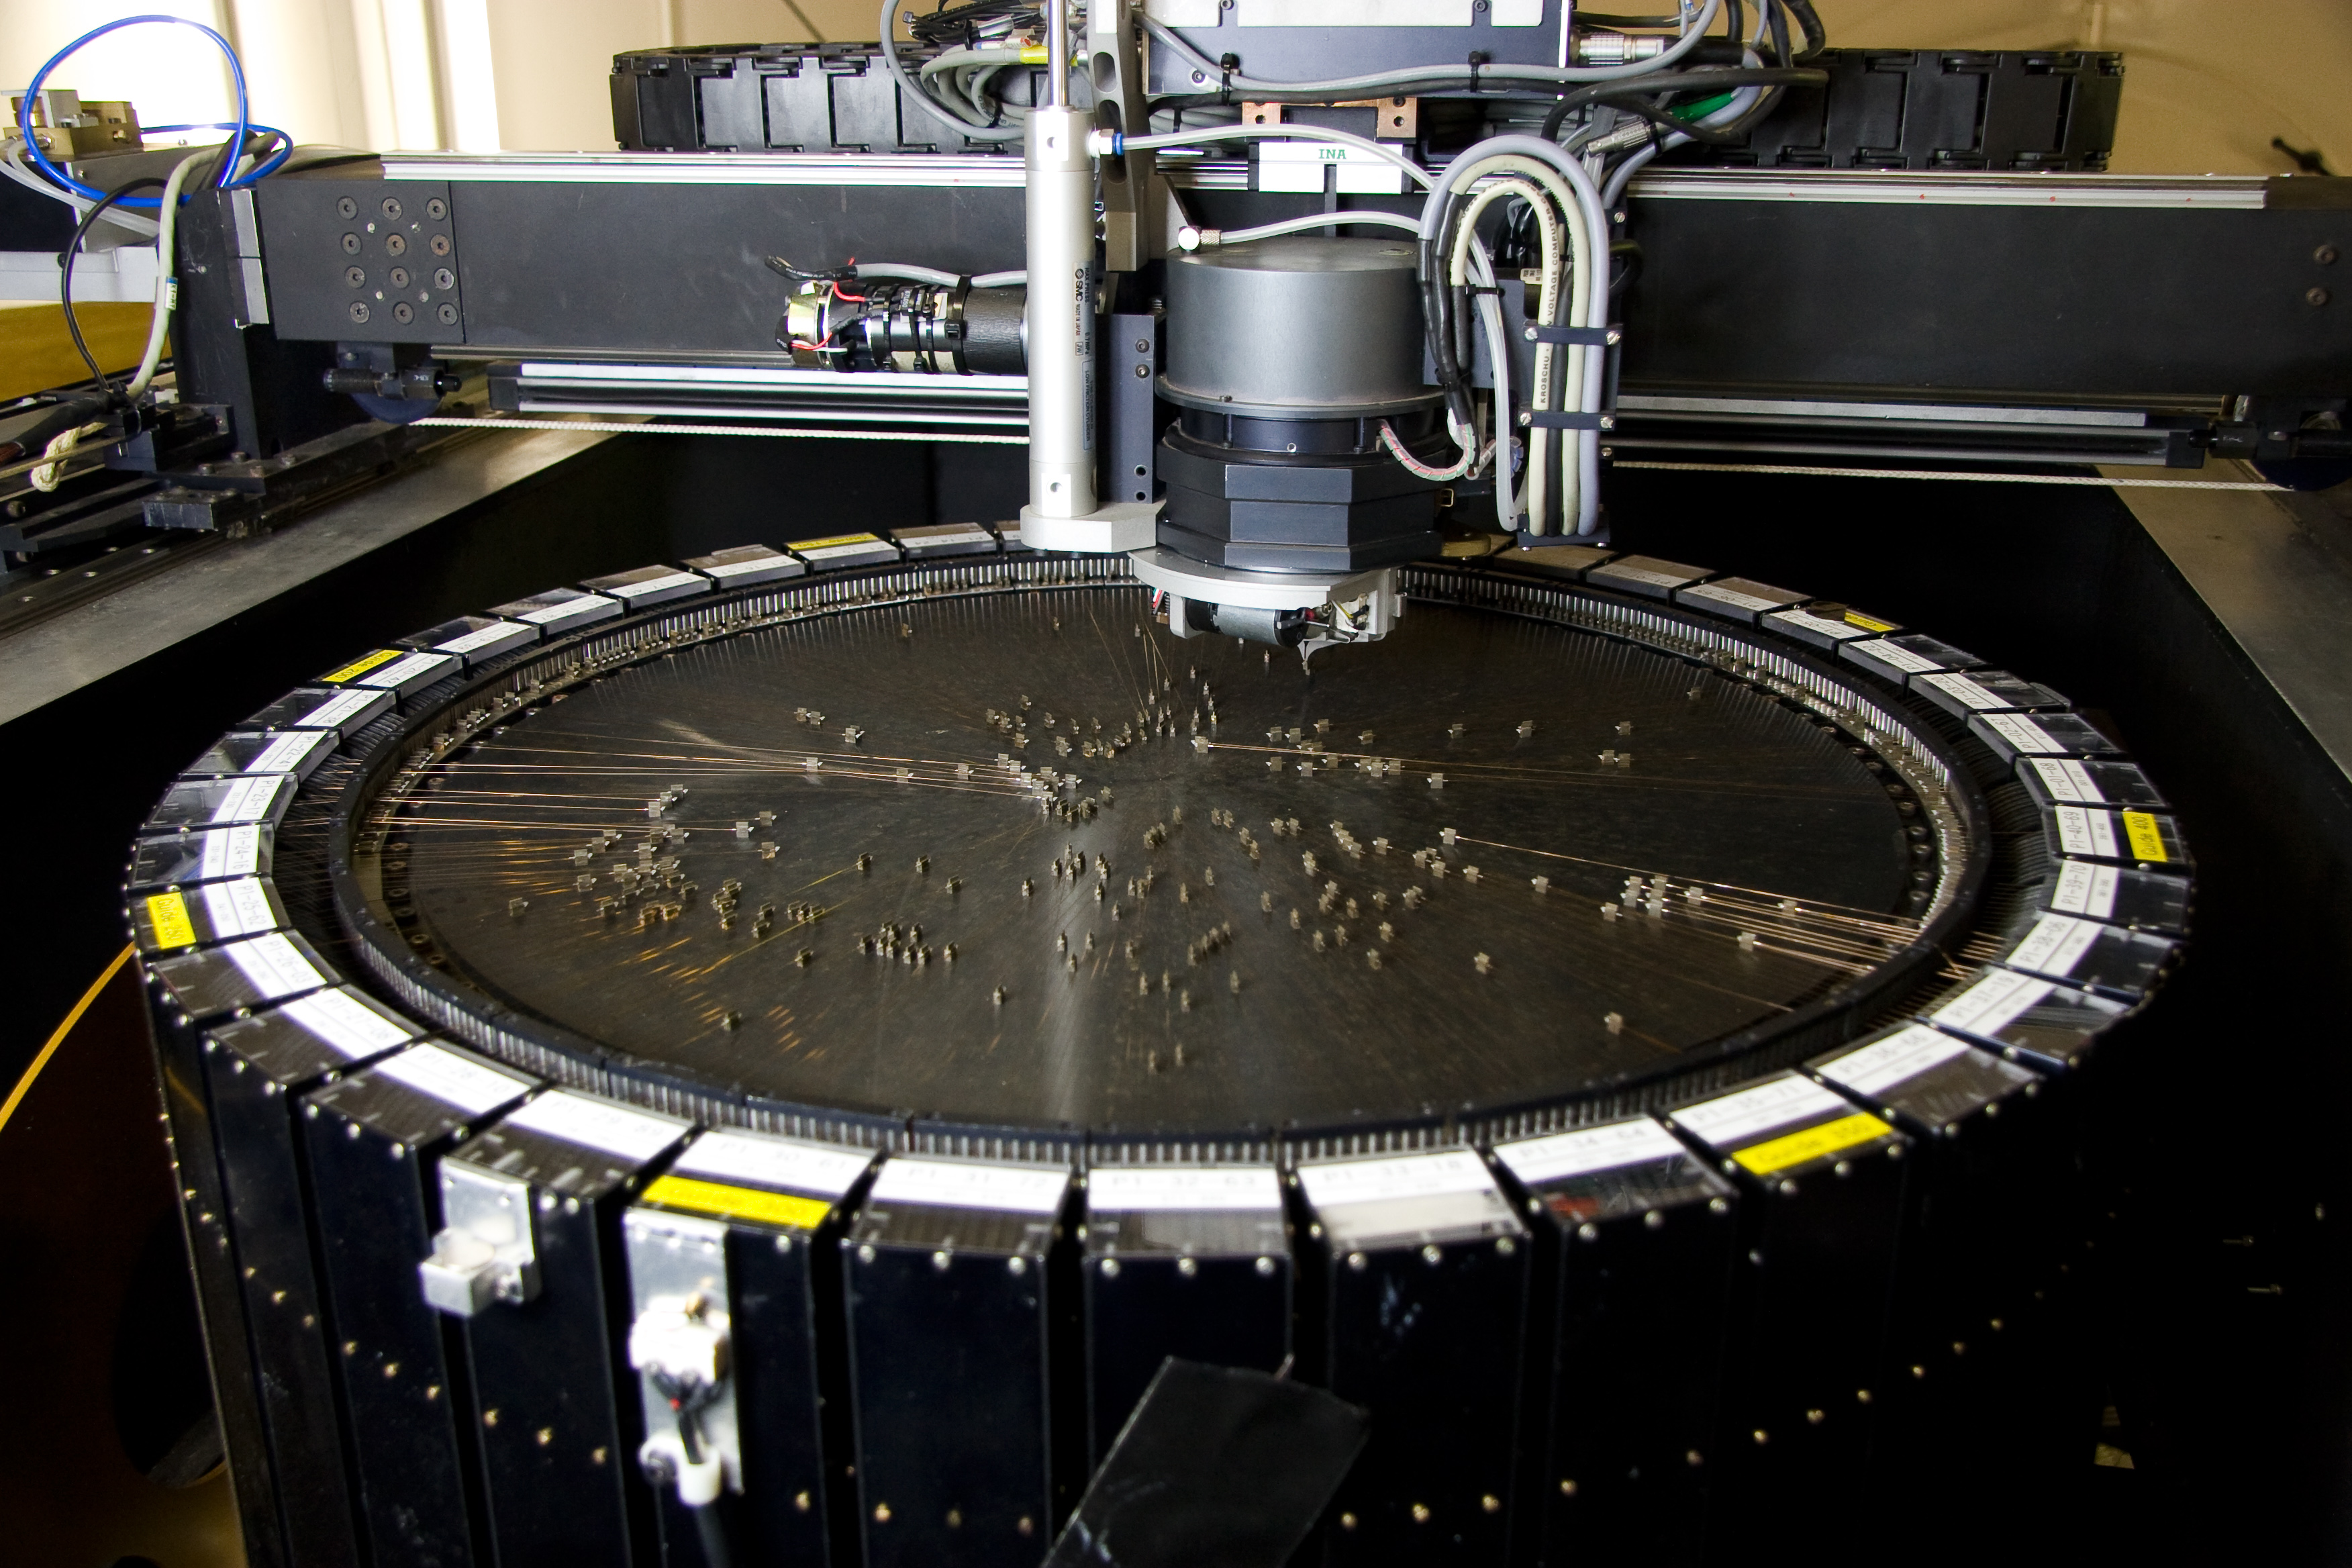
\includegraphics[height=50mm]{./plots/2df_spectrograph.jpg} \\
\end{tabular}
\caption{The Anglo-Australian telescope (left) at the Australian Astronomical Observatory (AAO) sheltered the 2DF instrument which consisted on a multi-fiber spectrograph called AAOmega. On the right is shown the focal plane where each fiber is moved individually to the image of the celestial object whose spectrum is to be extracted.}
\label{fig:2df_survey}
\end{figure}

In chapter~\ref{ch:odds} we use a derived galaxy catalog called the 2dF-SDSS LRG and QSO catalog (2SLAQ) \citep{Cannon2006} of about 13000 luminous red galaxies with good spectroscopic redshift quality as a trainning catalog where to calibrate our photo-$z$s.

\subsection{Sloan Digital Sky Survey (SDSS)}
\label{sec:sdss}
The Sloan Digital Sky Survey (SDSS) \citep{York2000} has been one of the more ambitious galaxy surveys carried out. It was performed in several phases: SDSS-I (2000-2005) and SDSS-II (2005-2008). Later the survey was extended until 2014 with a program called SDSS-III that lies beyond this work.

The SDSS used a dedicated 2.5-meter telescope~\citep{Gunn2006}, shown on the left of Fig.~\ref{fig:sdss_survey}, at Apache Point Observatory (APO), New Mexico, equipped with two special-purpose instruments. The first one is a 120-megapixel (24 2048$\times$2048 CCDs) camera~\citep{Gunn1998}, shown on the right of Fig.~\ref{fig:sdss_survey}, that imaged in drift-scan mode\footnote{The drift-scan technique makes use of the movement of the sky at the focal plane of a telescope when its drive is switched off, to image long continuous strips of the sky. Quite a big field can be explored almost automatically in this way.} 1.5~sq.~deg. of sky at a time in five broad bands $ugriz$ \citep{Fukugita1996}, whose throughput is shown in Fig.~\ref{fig:sdss_filt}. The photometry is calibrated to an AB system \citep{Oke1983}, and the zero points of the system are known to 1\%-2\% \citep{Abazajian2004} for the Data Release 7 (DR7) used in this thesis. The 95\% completeness magnitude limits of the images are 22.0, 22.2, 22.2, 21.3 and 20.5, respectively for \textit{ugriz} \citep{Abazajian2004}, although these values depend, as expected, on seeing and sky brightness. The second instrument is a 640-fiber-fed pair of multiobject double spectrographs, giving coverage from 3800~\AA \ to 9200~\AA \ at a spectral power resolution\footnote{The spectral power resolution of an spectrograph is a measure of its ability to resolve features in the electromagnetic spectrum. It is quantified as $R \equiv \lambda / \Delta \lambda$ where $\Delta \lambda$ is the smallest difference in wavelengths that can be distinguished at a wavelength of $\lambda$.} of $R\simeq$~2000, which measured spectra of more than 600 galaxies and quasars in a single observation. 

The SDSS-II final Data Release 7 (DR7)~\citep{Abazajian2009} has provided multi-color images in a high-latitude region in the Northern Galactic Cap for a total of $\sim$230 million celestial objects within a sky area of 8423~sq.~deg., together with spectroscopy of complete samples of galaxies and quasars covering about 8200~sq.~deg., what is refered as the Legacy survey. Additionally, it has also imaged 3240~sq.~deg. of sky at lower Galactic latitudes providing data for 127 million distinct objects (including many stars at low latitude) to study the structure of the Milky Way, what is refered as the SEGUE (Sloan Extension for Galactic Understanding and Exploration) survey \citep{Yanny2009}. The catalog derived includes more than 350 million celestial objects, and spectra of 930,000 galaxies, 120,000 quasars, and 460,000 stars. The data are fully calibrated and reduced, carefully checked for quality, and publically accessible on the web through the Catalog Archive Server (CAS) \citep{Thakar2008}. 
\begin{figure}
\centering
\begin{tabular}{rl}
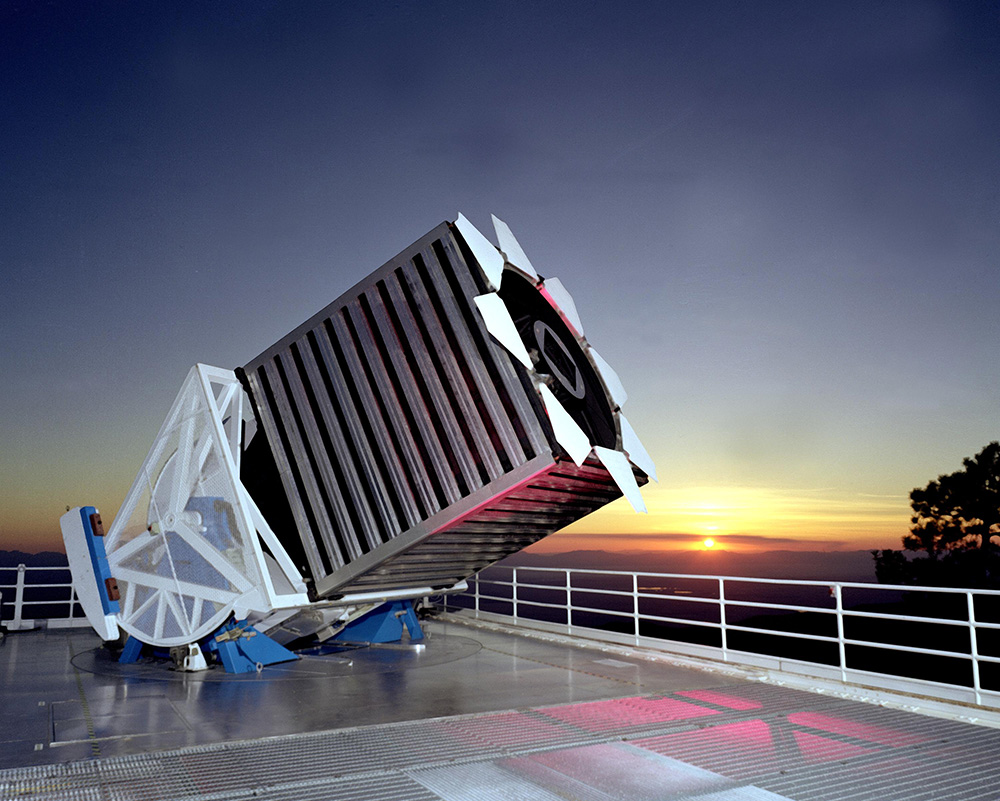
\includegraphics[height=50mm]{./plots/sdss_telescope.jpg} & 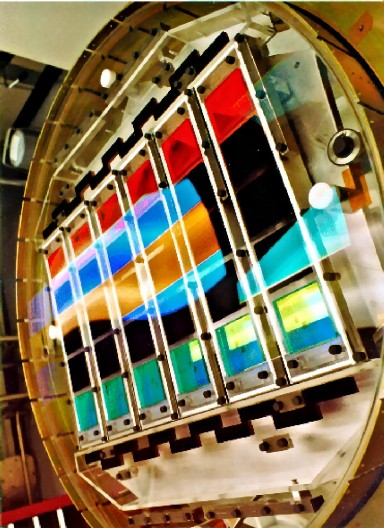
\includegraphics[height=50mm]{./plots/sdss_camera.jpg}
\end{tabular}
\caption{The SDSS 2.5m telescope (left) at the Apache Point Observatory (APO) shelters the SDSS CCD imaging camera (right) covered by five broad bands \textit{ugriz} whose throughput is shown in Fig.~\ref{fig:sdss_filt}.}
\label{fig:sdss_survey}
\end{figure}

Some derived galaxy catalogs have been built from the SDSS data, such as the Mega-Z LRG galaxy catalog \citep{Collister2007}, that we use in chapter~\ref{ch:odds}, which consists of a selection of $\sim1$~million LRGs in the redshift range $0.4<z<0.7$ with limiting magnitude $i_{AB}<20$. A much reduced version of the Mega-Z catalog called the 2dF-SDSS LRG and QSO catalog (2SLAQ) \citep{Cannon2006} with matched spectroscopic information from the 2-degree Field Galaxy Redshift Survey (2dFGRS) has been produced and it can be used to calibrate and train photo-$z$ methods for the photo-$z$ determination of the Mega-Z galaxies. It is composed of a total of $13100$ luminous red galaxies along a strip of $2$~deg width along the celestial equator. A map of the Mega-Z and 2SLAQ galaxies on the sky can be found in Fig.~\ref{scatter_map} in blue and red respectively.

\subsection{Physics of the Accelerating Universe at the William Herschel Telescope (PAU@WHT) Survey}
\label{sec:pau}

The Physics of the Accelerating Universe survey at the William Herschel Telescope (PAU@WHT) will start mapping a small area of the sky ($\sim$200~sq.~deg) in the fall of 2014 using a new technique to determine redshifts semi-spectroscopically. It consists of a photometric system composed of 40 narrow bands of $\sim$125\AA \ width (bottom of Fig.~\ref{pau_theo_bands}), plus six broad bands $ugrizY$ (top of Fig.~\ref{pau_theo_bands}), similar to the ones on the SDSS instrument.

The PAU instrument (PAUCam; \citet{Castander2012}), shown on the right of Fig.~\ref{fig:pau_survey}, will be located at the prime focus of the 4-m diameter William Herschel Telescope (WHT) (left of Fig.~\ref{fig:pau_survey}), in the Observatorio del Roque de los Muchachos (ORM observatory) in La Palma. Simulations indicate that PAUCam at the WHT will be able to image about 2 square degrees per night with the 40 narrow and broad bands up to an AB magnitude depth of $i\sim22.5$, providing low-resolution spectra ($R$$\sim50$) for around 30000 galaxies, 5000 stars and 1000 quasars per night.
\begin{figure}
\centering
\begin{tabular}{rl}
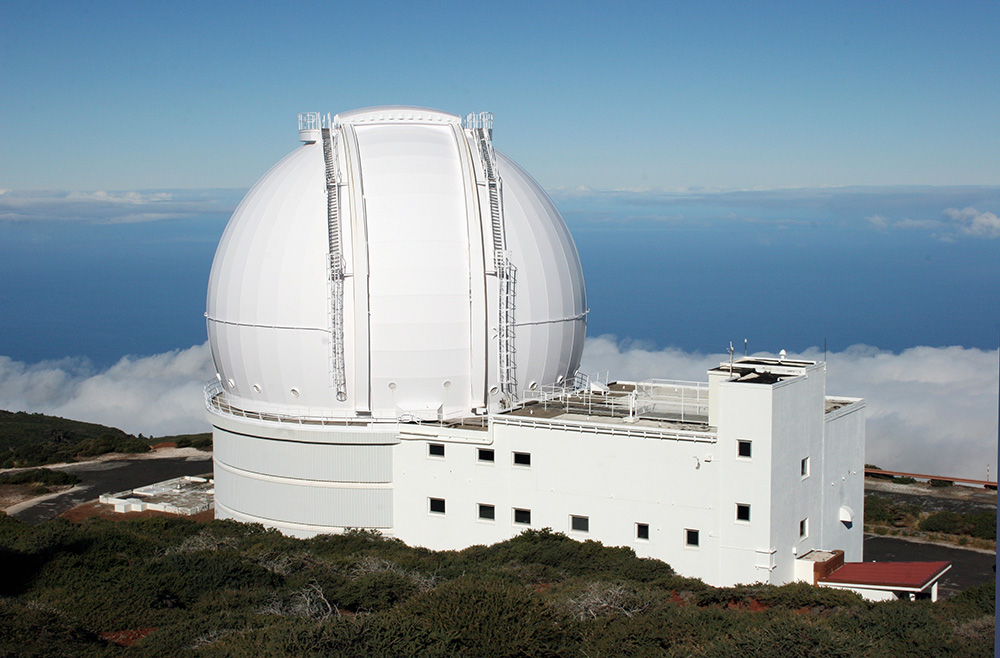
\includegraphics[height=50mm]{./plots/pau_telescope.jpg} & 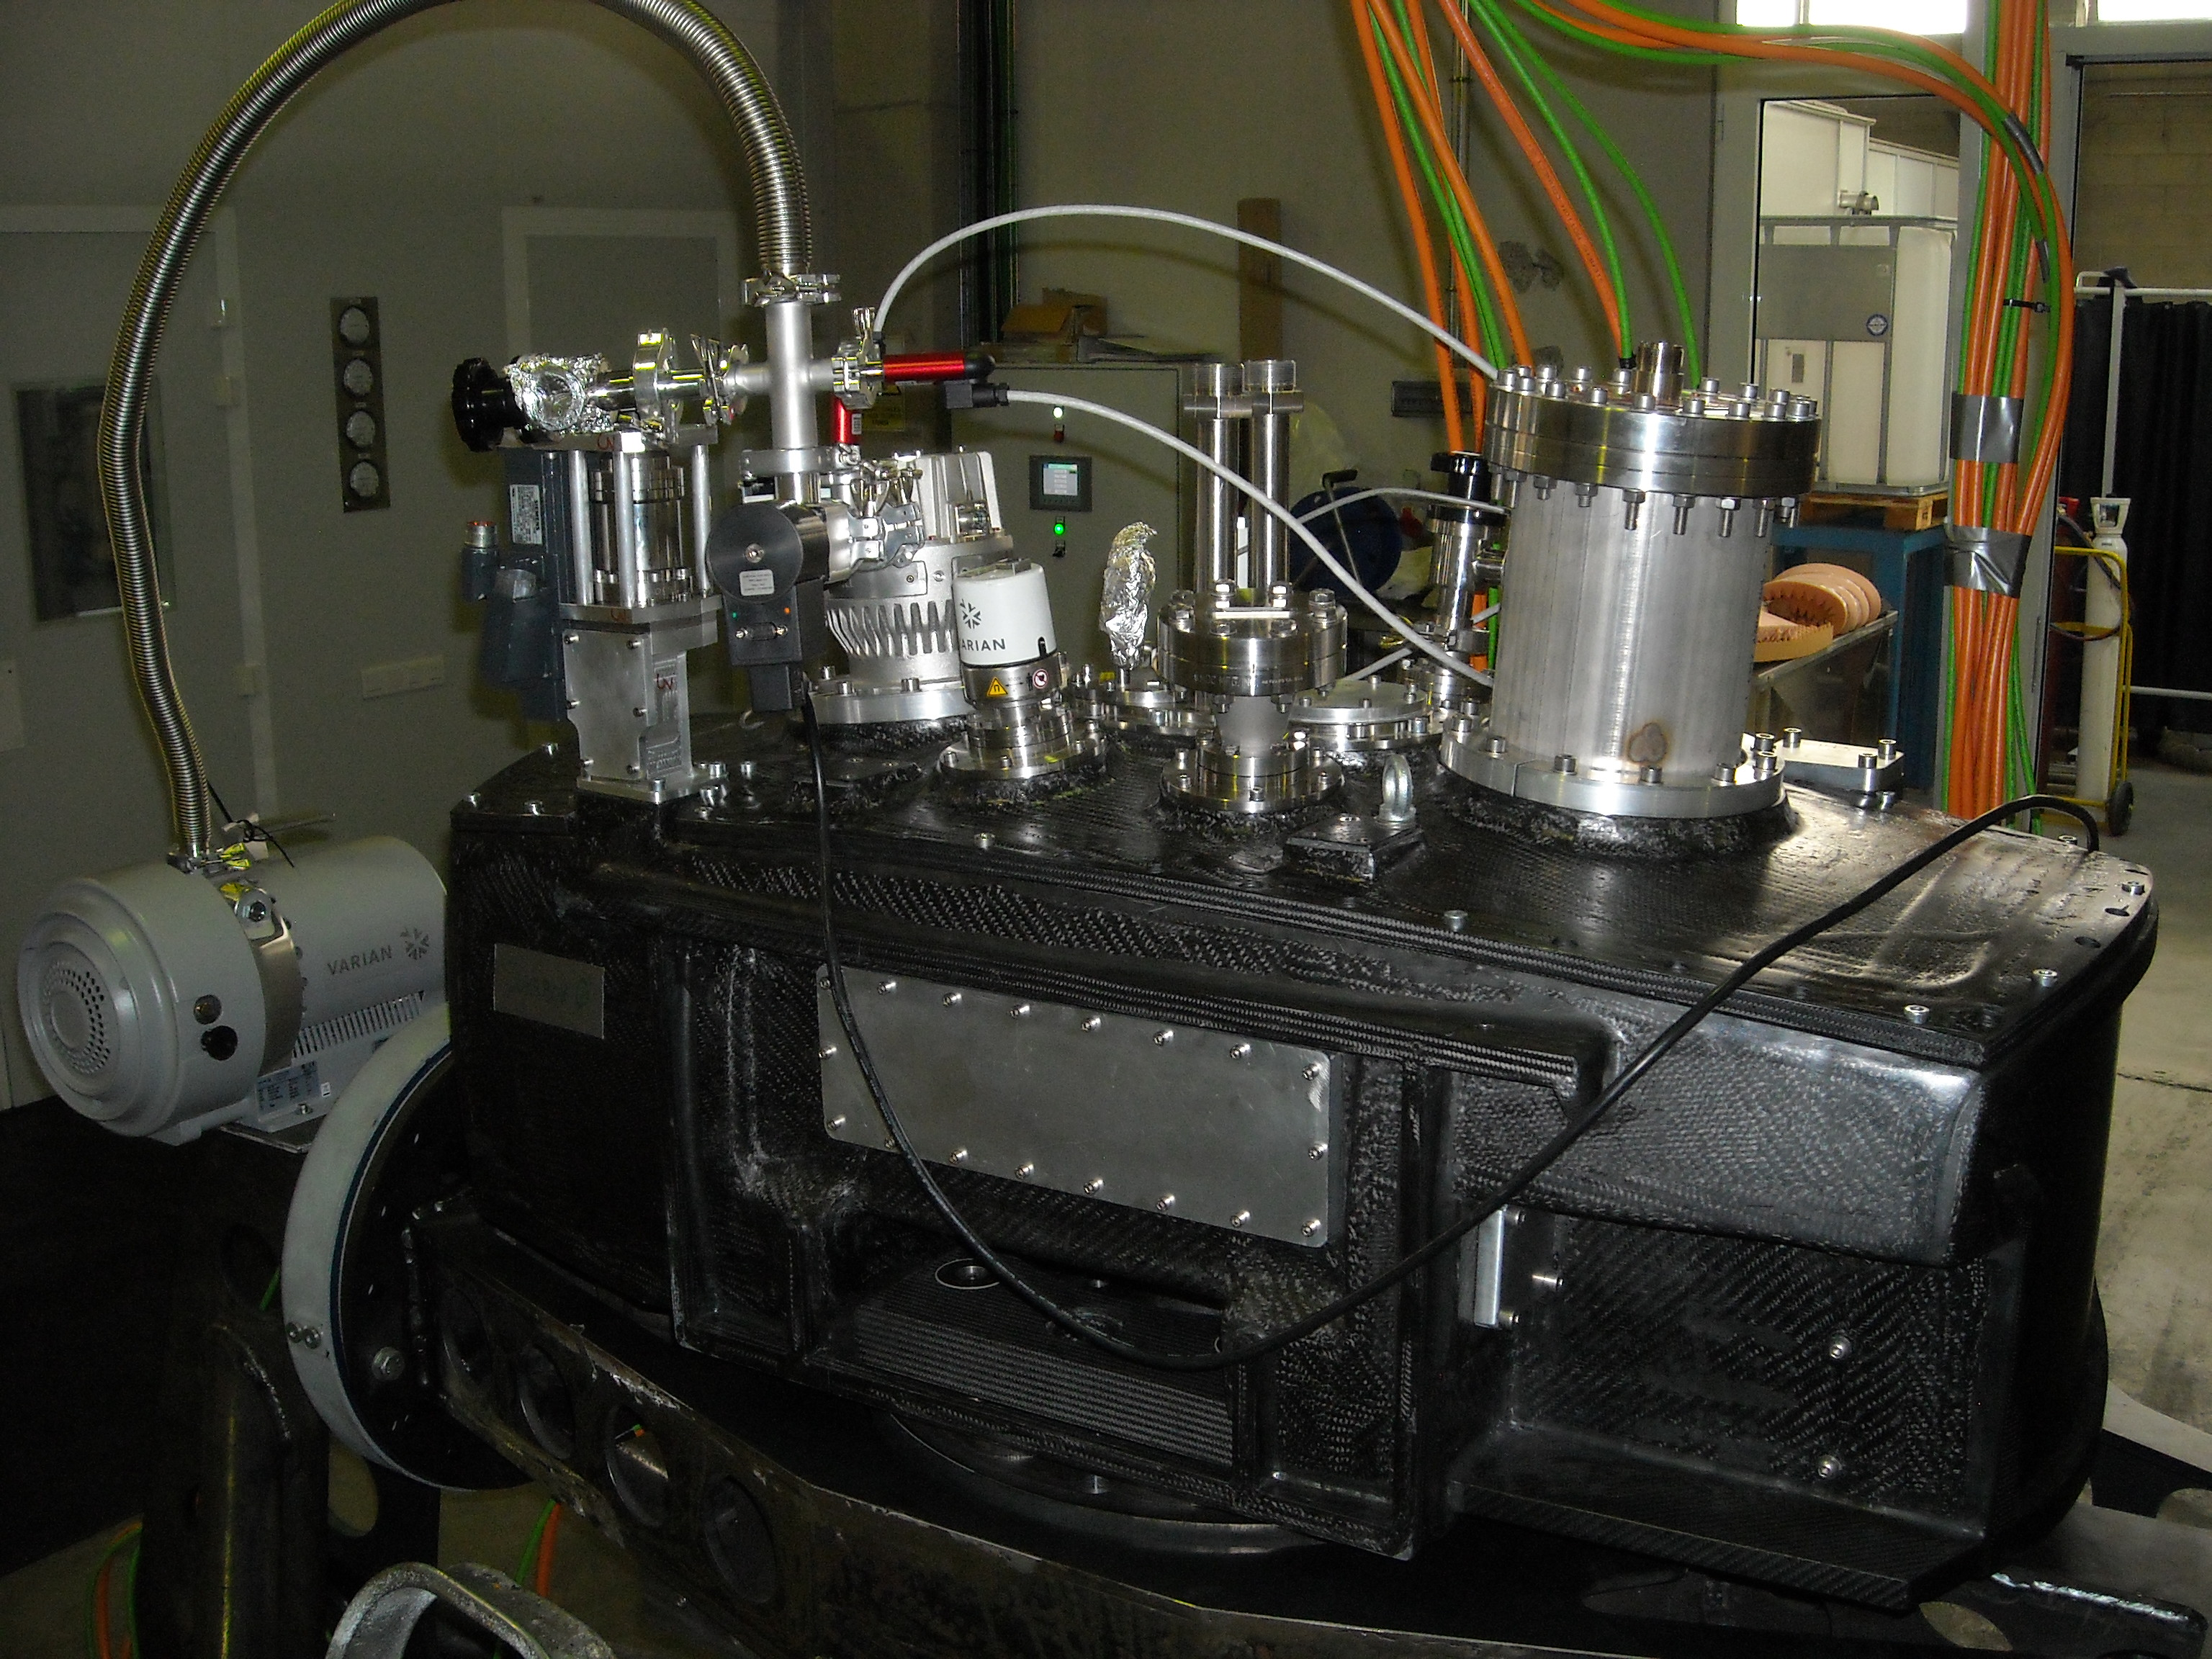
\includegraphics[height=50mm]{./plots/paucam.jpg}
\end{tabular}
\caption{The William Herschell Telescope (WHT) dome (left) which will shelter PAUCam (right) whose photometric system is composed of 40 narrow bands.}
\label{fig:pau_survey}
\end{figure}

Originally, in \citet{Benitez2009}, the PAU Survey was intended to be a larger survey covering about 8000~sq.~deg. of the sky to measure Baryonic Acoustic Oscillations (BAO) on the transversal (or angular) and radial (or the line-of-sight) directions. Measuring BAO transversally does not suppose any challenge, since only the angular coordinates of the galaxies on the sky must be known with a precision not necessarily better than $\sim0.1$~deg (any telescope has a better angular resolution). However, detecting the BAO signature on the radial direction involves measuring the distance to galaxies, and therefore the redshift, with a precision of at least $\sigma_z \sim 0.003(1+z)$, which cannot be achieved with conventional photometric surveys. \citet{Benitez2009} shows that a precision better than this does not result in a significant improvement in the measurement of BAO, since the intrinsic width of the BAO signature of this size in redshift.

The PAU@WHT survey will, instead, study the properties of dark energy by cross-correlating measurements of Redshift Space Distortions (RSD), on a bright sample ($i_{AB}<22.5$), and Weak-Lensing Magnification (MAG), on a faint sample ($22.5<i_{AB}<23.7$), over a reduced area of the sky. \citet{Gaztanaga2012} shows that such measurements, even done in a more moderate area, can provide useful information about the nature of dark energy. Measurements of RSD also require a redshift precision of at least $\sim 0.003(1+z)$. 

When not in use by the PAU team, PAUCam will be used as a community instrument, able to provide spectral energy distributions (SED) of moderate resolution for a very large sample of objects, allowing the study of a variety of scientific topics beyond cosmology. 
